\chapter{Derivation of spreading coefficient limit of declining infection}\label{chap:principles}

In this document I try to develop a model that would help me to understand the
essential figures and numbers that we should be monitored and measured in order to 
distinguish the effective and ineffective measures in limiting the spread of
the COVID19 virus.

I start the derivation from the measured reproduction number $R0$. We know that
the nature of the growth of the infection is exponential which inherently
means the disease is spread by infected persons infecting the uninfected ones
over certain period of time.

With COVID19 there is lots of statistics about number of
infected persons, daily new cases, deaths and recoveries. Based on these
statistics we may derive the estimate of the contamination time during which
the infected patient spreads the disease in such a manner that the daily
proportional growth equals the monitored reproduction number.

Under assumption that infected persons spread the disease with constant
fraction of cases per day, the newly infected persons tomorrow can be
expressed as
\begin{align}
    y\left(n\right)&=K y\left(n-1\right)\\
    K&= \frac{y\left(n\right)}{y\left(n-1\right)}=
    \frac{y\left(n\right)-y\left(n-1\right)}{y\left(n-1\right)}+1
\end{align}
where $y\left(n\right)$ is the number of infected persons on day $n$. Without
limiting measures $K$ is assumed here to be relatively constant. 

We may express $K$ as
\begin{align}
    K&= 1+S\\
    S &= \frac{y\left(n\right)-y\left(n-1\right)}{y\left(n-1\right)},
\end{align}
where $S$ is spreading coefficient, the \emph{ ratio of of daily increase of
    cases  to
active cases }. It should be noted that any estimation error that is in fixed
proportion to actually confirmed cases is canceled in calculation of $S$. Thus
we can state that any measure that gives us proportionally relatively stable
information will provide us accurate information about $S$.

As shown before, $K_l$ and $S$ can be measured. So can be the reproduction
number $R_0$, which for the COVID19 have been estimated to be $R_0=2.06 \ldots
2.52$~\cite{Zhang_S2020}.
These two expansion mechanisms are related, ans they should match at least in early phases of
epidemic, when deaths, recoveries, countermeasures, and developing immunity do not hinder the
spreading. The relation can be expressed as 
\begin{align}
    K^{T_c}&= 1+R_0\\
    T_c&=\frac{\ln\left(1+R_0\right)}{\ln\left(K\right)},
\end{align}
where $T_c$ is the contamination time, i.e.\ the effective time during which the patients
spread the disease. It can be thought as a time before patient get's so
visibly sick that he will be isolated/quarantined from the community and thus
does not spread the disease. This time is specific to disease and we may
assume here it is relatively constant.

We may now denote the spreading coefficient, measured as the ratio of increase
to the active cases, in the beginning of the epidemic as $S_0$. Thus
\begin{align}
    T_c&=\frac{\ln\left(1+R_0\right)}{\ln\left(1+S_0\right)}
\end{align}
For present COVID19, $S_0$ seems to be, with reasonable number of cases,
between 0.3 and 0.2, thus we may use $S_0=0.25$ in our example
calculations. We may now preform an example calculation for contamination
period 
\begin{align}
    S_0&=0.25\\
    R_0&=2.5\\
    T_c&=\frac{\ln\left(1+R_0\right)}{\ln\left(1+S_0\right)}=5.6.
\end{align}
Thus the estimate of the contamination time is 5.6 days, and we assume that to
remain constant.

Under ongoing epidemic, public authorities and private persons perform
measures to reduce $S$ in order to hinder the spread of the disease. However,
as $S$ and $R_0$ are connected, we may try to calculate \emph{how low we should
reduce $S$ in order to stop the epidemic under assumption that $T_T$ does not
change}. Stopping the epidemic means $R_0< 1$. We may now calculate the limit
$S_l$ that should result in declining numbers of active patients.
\begin{align}
    {\left(1+S_l\right)}^{T_c}&<2\\
    S_l&<2^{\frac{\ln\left(1+S_0\right)}{\ln\left(1+R_0\right)}}-1.
\end{align}
With the given values for current COVID19 outbreak $S_l<0.13$. 

In Table~\ref{tab:variants} the obtained values under various assumptions are
presented.
\begin{table}[h!]
  \begin{center}
      \caption{Spreading coefficient limit value under various assumptions on
      reproduction number $R_0$ and initial spreading coefficient $S_0$}\label{tab:variants}
   \begin{tabular}{c|c|c|c} % <-- Alignments: 1st column left, 2nd middle and 3rd right, with vertical lines in between
        \textbf{$R_0$} & \textbf{$S_0$} & \textbf{$T_c$} & \textbf{$S_l$}\\
      \hline
      2 &0.25&4.9&0.15 \\
      2 &0.3&4.2&0.18\\
      2 &0.4&3.7&0.21\\
      2.5&0.25&5.6&0.13\\
      2.5&0.3&4.8&0.16\\
      2.5&0.4&4.2&0.18\\
      3 &0.25&6.2&0.11\\
      3 &0.3&5.3&0.14\\
      3 &0.4&4.6&0.18\\
    \end{tabular}
  \end{center}
\end{table}
These values reveal that with given parameter spread there is no
\emph{practical} difference in contamination time, it lies between 3.7 to 6.2
days. This means practically two days difference, easily masked by individual
variation and real life uncertainties. 
Furthermore we may quite
certainly say there is no chance of epidemic to stop with spreading factors
larger than 0.2. Assuming 0.15 might be wishful thinking but may work, and 0.1 should be
quite safe. 

As the global data for the cases have been collected and made generally
available it is possible to evaluate the theory by comparing it to
existing data. That comparison well be presented in Chapter~\ref{chap:observations}.

\section{Parameter estimation with measured data}
On March 23 friend of mine,  Teemu Lehtimäki suggested that the measured
relative growth e.g.\ in Sweden and the trend of measured cases do not support
the $R_0$ parameter value 2.x, but that the correct number could be higher. The
arising is, what is the most reliable way to estimate $T_t$ in the beginning
of the epidemic, when the behaviour of the individuals is not affected by the
counter measures, but when the cases are relatively scarce. I think one
possible 
method is LMS curve fitting based on measured relative growth and difference
of cases $y\left(n\right)-y\left(n-x\right)$. 

\chapter{Discrete time infection system model}
In order to gain more insight on input-output relation (i.e the
transfer function),,stability and critical parameters to be identified, I
developed s simple discrete-time system model.

Fig \ref{fig:infection_system} depicts a discrete time infection system model
in Z-domain. $X(Z)$ are the
    the infectious patients entering the community with spreading factor $S$.
$X_q(Z)$ are the infectious patients entering the system through
quarantine. They are known to be infectious, but they are isolated.
\begin{figure}
    \centering
    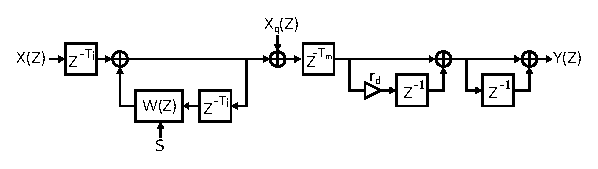
\includegraphics[width=\textwidth]{Figures/Infection_system.eps}
    \caption{Discrete time Infection system in Z-domain.}\label{fig:infection_system}
\end{figure}

Fig \ref{fig:infection_feedback_system} presents the infection feedback
eventually causing the exponential growth. Every infectious patient $X$ will
initiate an infection chain over $T_c$ days, adding $S$ new infections. 
\begin{figure}
    \centering
    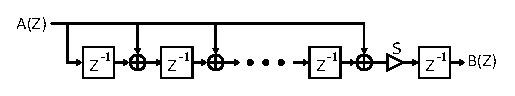
\includegraphics[width=\textwidth]{Figures/Contamination_feedback_system.eps}
    \caption{Infection feedback system $W(Z)$}\label{fig:infection_feedback_system}
\end{figure}

Due to the feedback through $W(Z)$, the system will eventually have positive
feedback causing exponential type of growth. The parameters characterizing the
system behaviour are listed in Table \ref{table:system parameters}
\begin{table}
    \centering
    \caption{Infection system parameters}
    \begin{tabular}{l|p{10cm}}
        \textbf{Parameter} & \textbf{Description} \\
        \hline
        $S$ & Spreading factor.\\
        $T_i$ & Incubation period. It is assumed that the patient is not
        infectious during this time. \\
        $T_c$ & Contamination period. Patiend spreads the disease during this
        time until is isolated from the population because of sickness or
        treatment.\\
        $T_m$ & Monitoring delay. The time from the patient becoming
        infectious to registration of the case.\\
        $r_d$ & Death rate. The share of the registererd patients dying.\\
        $T_d$ & Delay of death. Time from registration to death.\\
        $T_r$ & Recovery time.
    \end{tabular}
    \label{tab:system_parameters}
\end{table}

The parameter $S$, is multiplying the sample stream in feedback system
$W(Z)$. Therefore following observations about the nature of the
system can be made.
\begin{itemize}
    \item System is not linear time invariant, but can be considered piecewise
        linear over
        the coherence time on $S$, i.e. during the periods $S$ is not altered,
        and linear time invariant, if $S$ is considered constant.
    \item As the fraction of recovered and dead patiences increases, the $S$
        is decreased. This phenomenon is not included in this model,
        indicating infinite population.
    \item Timing relation of the signal and $S$ in the feedback path indicates
        that the effect of changes in policies affecting $S$ are immediate to
        the spreading of the disease, and visible in the statistics after the
        measurement delay $T_M$.
\end{itemize}

